\section{La plateforme Eclipse}

Avant de parler de fragmentation en plugins, il est important de définir le fonctionnement d'Eclipse.

\subsection{Historique}

Créée en 2001, le but du projet Eclipse était de fournir un socle pour la création d'environnements de développement.
\subparagraph*{}
En 2004, lors du lancement d'Eclipse RCP\footnote{Rich Client Platform}, l'objectif du projet a été étendu pour prendre en compte l'utilisation du framework Eclipse par des applications clientes.
Au départ, Eclipse était conçu pour créer un environnement de développement Java autour duquel aurait été construit d'autres applications.
Finalement, la base est conçue comme un framework utilisable pour des développements d'applications clientes dîtes riches.

\subsection{Principe}

Eclipse est une plateforme composée de plugins qui interagissent les uns avec les autres (figure \ref{PlatformEclipse} p.\pageref{PlatformEclipse}).
La plateforme Eclipse est fournie avec un framework minimaliste appelé ``Runtime''. Contrairement à une application extensible qui est composée d'une gros framework commun.
Autour de ce framework d'autres plugins sont déployés afin de permettre la création d'une application riche.
Exemple : 
\begin{itemize}
  \item SWT : création de composants graphiques
  \item JFace : création de composants plus riches basés sur SWT
  \item Workbench : gestion de l'environnement de travail (menu, action, \ldots)
\end{itemize}

Cette plateforme basée sur l'extensibilité est réalisée grâce au mécanisme de points d'extension.

\begin{figure}[!h]
\begin{center}
  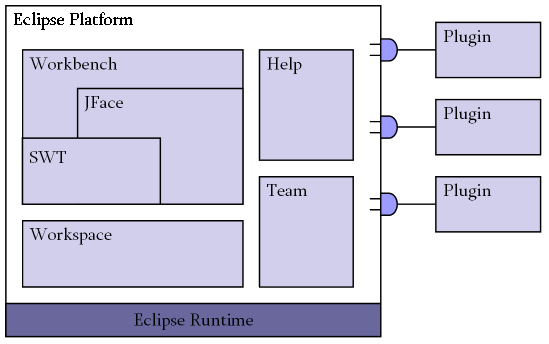
\includegraphics[scale=.55]{images/archi_eclipse_platform.png}
  \caption{Diagramme représentant une plateforme Eclipse}
  \label{PlatformEclipse}
\end{center}
\end{figure}

\subparagraph*{}
Le framework de base sert de conteneur pour les extensions.
Toutes les fonctionnalités sont développées dans des <<plug-in>> (Bundles).
Cela offre l'avantage d'être ouvert et transparent. 
Il est par exemple plus facile de remplacer une fonctionnalité par une autre.

\subparagraph*{}
Une application basée sur Eclipse utilise le registre d'extension et les services OSGI\footnote{Open Services Gateway initiative}.
Ce standard permet de gérer les dépendances de plugin et l'extensibilité de l'application.
Il évite aussi le couplage des modules Java.
Pour modulariser l'application, il suffit d'utiliser les ``features'' Eclipse.

\subparagraph*{}
Une feature Eclipse permet de déployer des plugins différemment suivant le client ou suivant la plateforme cible.

\subsection{Déploiement d'un plugin sur une plateforme Eclipse}

La plateforme Eclipse implémente le mécanisme de mise à jour d'une application que l'on retrouve sur quasi tous les logiciels.
Dans Eclipse un plugin peut être déployé par un ``update-site''.

\subparagraph*{}
En réalité, un ``update-site'' déploie des ``features'' composées de ``plugins'' (figure \ref{figure:EclipsePlatformDeploiement} p.\pageref{figure:EclipsePlatformDeploiement}).
Le mécanisme d'installation, vérifie en fonction des plugins requis par la feature à installer si la plateforme Eclipse les possède.
En cas d'échec les plugins ne sont pas installés.

\begin{figure}[!h]
\begin{center}
  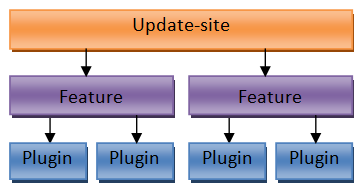
\includegraphics[scale=.55]{images/archi_eclipse_deploiement.png}
  \caption{Architecture de déploiement d'un plugin sur la plateforme Eclipse}
  \label{figure:EclipsePlatformDeploiement}
\end{center}
\end{figure}

\subsection{Structure}

Cette partie définie la composition des différents éléments Eclipse : Plugin et feature.

\subsubsection{Feature}

Une feature est gérée par un fichier \texttt{feature.xml} qui contient au format XML, la liste des plugins composants la fonctionnalité.

\subsubsection{Plugin}

L'administration des plugins est gérée par OSGI, qui utilise le fichier \texttt{MANIFEST.MF} contenu dans la structure du plugin. 
C'est ce fichier qui permettra de gérer les dépendances de plugins.

Quant à Eclipse, la plateforme utilise entre autre le fichier \texttt{plugin.xml}.
Ce fichier contient les données XML de construction de l'interface utilisateur.
On peut y déclarer des actions, des menus, des vues, des éditeurs, \ldots

\subsubsection{OSGI}\label{OSGI}

Eclipse utilise le framework OSGI, qui permet de gérer le chargement des classes, l'administration des plugins et les dépendances entre eux. 
Pour généraliser, ce framework Java gère le cycle de vie d'une application, les services, un environnement d'exécution et des modules.
